\documentclass{article}

\usepackage[a4paper, total={6.2in, 8in}]{geometry}
\usepackage{pgfplots}
\pgfplotsset{compat=1.18}
\usepackage{graphicx}
\usepackage{array}
\usepackage{hhline}
\usepackage{subcaption}
\usepackage{lipsum}
\usepackage{blindtext}
\usepackage{titlesec}

\setlength\parindent{0pt}

\title{\LARGE\bfseries An Assessment of the Potential Behaviours of Self-Driving Cars}
\author{Luke Guppy \\
$3^{rd}$ Year 2023-2024 \\
Supervisor: Andrew Hague}
\date{}

\begin{document}

\maketitle

\newpage
\tableofcontents
\newpage

\section*{Abstract}
This project explores the implementation of curriculum learning to train self-driving cars within a realistic driving simulation environment developed in Unity using the ML-Agents package. The objective is to train an autonomous agent with the ability to navigate an environment while adhering to traffic rules and avoiding collisions. The simulation incorporates various elements such as traffic lights, lane centering, corner slowing, and path following, all integral components of a comprehensive curriculum aimed at progressively teaching the agent to drive safely and efficiently.\\

Throughout the development process, multiple stages of reward systems were devised and iteratively refined to incentivise desired behaviours, ultimately culminating in the creation of a successful framework. The resulting agent demonstrates proficient path following capabilities, effectively negotiating complex scenarios while following traffic regulations.\\

This project contributes to the advancement of autonomous vehicle technology by providing insights into the effectiveness of curriculum learning methodologies for training self-driving car agents. The modular nature of the simulation allows for flexible experimentation and evaluation of various training strategies, paving the way for further research in this domain. It also gives a strong insight as to how a reward system can be developed to iteratively implement new behaviours.

\subsection*{Keywords}
Self-driving cars, Reinforcement learning, Autonomous agents, Simulation environments, Curriculum learning, Traffic simulation, Agent-based modeling, Reward optimisation

\section{Introduction to the Project}
\lipsum[2][1]

\subsection{Refined Problem Statement and Addressed Gap}
\lipsum[2][1]

\section{Background Research}
\lipsum[2][1]

\subsection{Extending AI-Driven Vehicle Research:}
This project represents a focused extension of existing research on AI-driven vehicles, rather than more generalised or specialised approaches. While prior studies have contributed valuable insights, they often lack a specific focus on scenarios with the highest collision rates, such as straight roads, cross-junctions, and T-junctions. By honing in on these critical driving situations, this research aims to improve our understanding of how AI-driven cars navigate and adapt, particularly in the presence of human behaviors. 

\subsection{Areas Of Research:}
Key areas of research:
\begin{itemize}
    \item Road sections with the highest collision rates \cite{accident-types-and-causes}
    \item Human factors which cause the most incidents \cite{accident-types-and-causes} \cite{gov-crash-stats} \cite{Crash-human-causes}
    \item Existing reward functions for driving simulations \cite{Predictive-reward-function-for-ai-driving} \cite{Racing-reward-functions} \cite{Deep-RL-for-racing-driving} 
    \item Sensory inputs and visualisation of the environment \cite{General-overview-of-ai-driving}
    \item Inputs and outputs of neural networks for learning in automated vehicles \cite{Collision-avoidance-in-lane-free-traffic-neural-system} \cite{Deep-RL-for-AI-driving-general-overview}
    \item Relationships between AI and human behaviours \cite{Collision-frequency-ai-and-humans} 
    \item Current progress and future plans for self-driving cars \cite{Deep-learning-for-AI-driving}
\end{itemize}

\subsection{Summary Of Research}
\subsubsection{Foundation}
The research started with a general overview of the current situation and progress of AI driving in the world. This meant understanding how sensors work, what features of the road the AIs use and other relevant features. It appears that there is a surprising number of sensors of various types: Cameras, Lidar, Radar, Ultrasonic, Infrared (for lanes) and GPS \cite{General-overview-of-ai-driving} which all have various strengths and weaknesses in the real world. In the simulation this can be heavily abstracted by the use of ray-casts and directly feeding information.

\subsubsection{Collision Occurrence}
\lipsum[2][1]

\subsubsection{Existing Implementations}
\lipsum[2][1]

\subsubsection{High Level Overview}
\lipsum[2][1]

\section{Technical Aspects}
\lipsum[2][1]

\subsection{Unity}

\lipsum[2][1]

\subsection{Unity Simulation Abstraction}
ML-Agents abstracts complex machine learning processes, simplifying their application within Unity so that it appears to be a black-box which you use methods to feed inputs and return outputs. This abstraction makes it only necessary to define reward structures, observations, and actions for agents without worrying about the intricacies of machine learning algorithms. For our project, this means we can create a realistic driving simulation with AI-driven cars navigating complex scenarios without getting bogged down in the technical complexities of machine learning.

\subsection{ML-Agents}
ML-Agents serves as a powerful bridge between machine learning algorithms and Unity-based simulations or games. Developed by Unity itself, this open-source python based package is tailored to integrate machine learning, specifically reinforcement learning, into Unity environments. As this project involves creating a simulated driving environment using Unity, ML-Agents is a natural fit.

\subsubsection{Reinforcement Learning Framework}
At the core of ML-Agents is a reinforcement learning framework. This framework allows developers to train intelligent agents through a process of trial and error, guided by a self-implemented reward system. In this project, the agent is the car, which will have the goal of training to reach a certain goal with the highest reward over time. However, it is strongly limited by the reward function which drastically impacts the behaviours it learns making it the most important aspect.

\subsubsection{Neural Network Policies}
ML-Agents employs the use of a neural network to model the policies of the agent. The neural network adapts and refines its parameters during training, optimising the decision-making process of the agent. In our case, the neural network will be crucial for teaching the AI-driven cars to navigate roads, respond to obstacles, and follow appropriate behavior at junctions. This is governed by the inputs which will be a series of sensory inputs, distances to checkpoint and any other inputs which may be added later.

\subsubsection{ML-Agents Algorithm}
To give an understanding of what applications would be successful to give the expected result, it's important to understand how these algorithms work. In the context of ML-Agents, the machine learning algorithms are primarily centered around Proximal Policy Optimization (PPO), a deep reinforcement learning algorithm. PPO strikes a balance between exploration and exploitation, allowing intelligent agents to learn optimal policies through trial and error within the simulated driving environment.\cite{PPO-MLAgents}\\

 The technical complexities lie in the architecture of the neural networks used to represent the agent, specifically tailored for PPO. These neural networks undergo iterative updates during training, incorporating advanced optimisation techniques associated with PPO. The objective remains to maximise the cumulative reward obtained by the agents over successive interactions with the environment.\\

 During training, PPO utilizes a trust region approach, ensuring that policy updates are performed within a constrained region to maintain stability and prevent abrupt changes. The trust region mechanism establishes constraints on the magnitude of policy updates during training. This ensures that the learning process occurs gradually, preventing drastic policy changes that might destabilise the training. By constraining policy updates, the trust region approach enhances the stability of the learning process and contributes to the algorithm's ability to adapt to varying conditions in the simulated driving environment in a more natural manner. This careful balance is crucial for achieving effective learning of complex driving scenarios and not learning drastic unpredictable behaviours.\\

 ML-Agents chose PPO based on research at Cornell University: ``Our experiments test PPO on a collection of benchmark tasks, including simulated robotic locomotion and Atari game playing, and we show that PPO outperforms other online policy gradient methods, and overall strikes a favorable balance between sample complexity, simplicity, and wall-time." \cite{PPO-Algorithms} This gives a reliable foundation of how PPO would effectively work in this environment.\\

 The technical complexities also extend to hyper-parameter tuning, where factors such as learning rates, discount factors, and exploration parameters play a pivotal role in optimising the training process. However these are set to default values which have been optimised by trial and error across many projects and editing them will likely have limited or even negative impacts.

\subsubsection{Non-Linearity In ML-Agents}
ML-Agents predominantly employs the Swish activation function for most of its neural network architectures, particularly for the hidden layers. Swish is a popular activation function that introduces non-linearity by smoothly blending the linear and nonlinear activations. Specifically, it is defined as $x*sigmoid(x)$ and avoids previous issues of other activation functions such as the vanishing gradient problem for $sigmoid(x)$. This problem occurs as the gradient tends to 0 with extreme values causing difficulties in gradient descent for learning and progressing towards the local maximum.\\ 

Swish allows neurons to output the relation with a smooth curve, promoting stronger gradients and potentially faster convergence during training. While other activation functions like tanh or sigmoid may also be utilized in specific cases based on the neural network architecture or task requirements, Swish serves as the default choice due to its efficiency in capturing complex relationships between inputs, thereby enabling the discovery of nonlinear patterns and the emergence of complex behaviors within the deep learning structure.\\

It was chosen by ML-Agents due to its promising results over these other popular activation functions as detailed by Google Brain in 2017.

\begin{figure}[h]
    \centering
    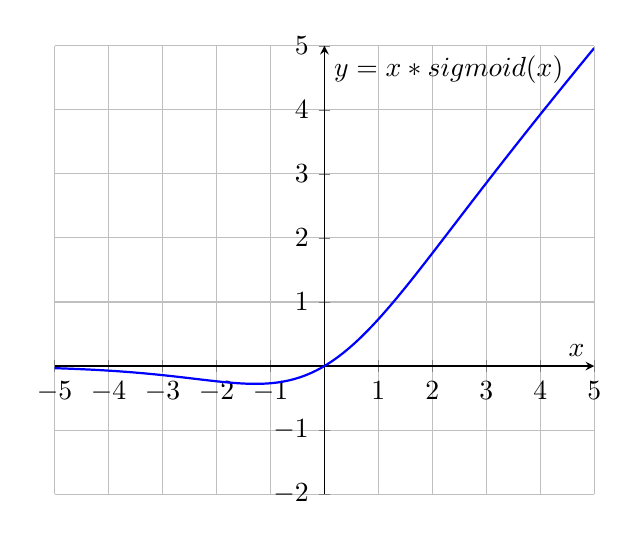
\begin{tikzpicture}
        \begin{axis}[
            xlabel=$x$,
            ylabel={$y = x*sigmoid(x)$},
            axis lines=middle,
            xmin=-5, xmax=5,
            ymin=-2, ymax=5,
            xtick={-5,-4,...,5},
            ytick={-2,-1,...,5},
            grid=both,
            domain=-5:5,
            samples=100,
            smooth,
        ]
        
        \addplot[blue,thick] {x * (1 / (1 + exp(-x)))};
        \end{axis}
    \end{tikzpicture}
    \caption{Swish Graph}
\end{figure}


\subsection{Community Support and Documentation}
ML-Agents benefits from an active community and extensive documentation, making it easy to implement and troubleshoot problems encountered with the project. The community support is invaluable for addressing challenges, seeking solutions, and staying updated on best practices during the development of the project.

\subsection{Git}
\lipsum[2][1]

\section{The Simulation Environment}
\lipsum[2][1]

\subsection{Roads}
\lipsum[2][1]

\subsection{Pathing}
\lipsum[2][1]

\subsection{The Car Control System}
\lipsum[2][1]

\subsection{Environmental Cars}
\lipsum[2][1]

\subsubsection{General Functionality}
\lipsum[2][1]

\subsubsection{Logical Implementation}
\lipsum[2][1]

\subsubsection{Traffic Light Interaction}
\lipsum[2][1]

\subsection{Traffic Light System}
\lipsum[2][1]

\subsubsection{Target Types}
\lipsum[2][1]

\subsubsection{Logical Implementation}
\lipsum[2][1]

\subsubsection{Smart Traffic}
\lipsum[2][1]

\section{The Agent}
\lipsum[2][1]

\subsection{Structure}
\lipsum[2][1]

\subsection{Controls}
\lipsum[2][1]

\subsection{ML-Agents Interaction}
\lipsum[2][1]

\section{Reinforcement Learning}
\lipsum[2][1]

\subsection{Reward Systems}
\lipsum[2][1]

\subsection{Curriculum Learning}
\lipsum[2][1]

\section{The Deep Neural Network}
\lipsum[2][1]

\subsection{Proximal Policy Optimisation}
\lipsum[2][1]

\subsection{Configuration}
\lipsum[2][1]

\subsection{Hyper-parameters}
\lipsum[2][1]

\subsection{Observations and Outputs}
\lipsum[2][1]

\section{Deep Reinforcement Learning}
\lipsum[2][1]

\section{Reward System}
\lipsum[2][1]

\subsection{Curriculum Learning Implementation}
\begin{itemize}
    \item What it is
    \item How it is being applied
    \item Behaviours being implemented
    \item Specific implementation
\end{itemize}

\subsection{Initial Reward System}
\begin{itemize}
    \item Weighted average
    \item Negative
    \item Issues with unpredicted behaviours
    \item Positive change
\end{itemize}

\subsection{Imitation Learning}
\begin{itemize}
    \item Graph for difference
    \item Reasons why non-imitation is better
    \item Using non-imitation for rest
\end{itemize}

\subsection{Final Reward System}
\lipsum[2][1]

\section{Problems and Oversights}
\lipsum[2][1]

\section{Conclusion}
\lipsum[2][1]

\section{Future Outlook}
\lipsum[2][1]

\section{Project Management}
\lipsum[2][1]

\section{Objectives}
\subsection{Must-Have Objectives:}
\begin{itemize}
\item \textbf{Develop a Realistic Simulation Environment:} Create a Unity-based simulation environment that abstracts real-world driving scenarios, focusing on essential features while omitting minor details.

\item \textbf{Design and Implement Learning Agents:} Develop reinforcement learning agents for the cars, ensuring they can navigate the simulation environment effectively and adapt to changing conditions.

\item \textbf{Conduct In-Depth Research:} Carry out comprehensive research on AI-driven cars, traffic dynamics, and human behaviour to inform the development of the simulation and learning agents.

\item \textbf{Training and Performance Analysis:} Train the AI agents and conduct rigorous performance analysis on the relevant features such as safety, speed, efficiency, and other metrics.

\item \textbf{Varied Situations:} Provide a series of different situations for learning (e.g., traffic lights, cross junctions, t-junctions, pedestrians) to challenge the AI cars to learn more general and applicable behaviours.

\item \textbf{Adapt Agent Based On Feedback:} Tweak and adjust the learning agent rewards depending on its results to better improve its learning capability.

\end{itemize}

\subsection{Additional Objectives (Exploration if Time Allows):}

\begin{itemize}

\item \textbf{Implement More Advanced Road Features:} Introducing more advanced situations such as roundabouts, overtaking or multi-lane roads to challenge the AI and further demonstrate AI-human interactions.

\item \textbf{Explore New Infrastructure:} Expand the simulation to explore potential new road infrastructure e.g., a lane specifically for AI, changing the speed limits for a simulation with only AI cars.

\item \textbf{Reinforcement Learning Optimisation:} Investigate techniques for optimising the machine learning models used by AI agents to adapt more effectively to dynamic road conditions.

\item \textbf{Traffic Optimisation Strategies:} Investigate strategies for optimising traffic flow and reducing congestion through the deployment of AI-driven cars, including adaptive traffic signal coordination and lane management.

\item \textbf{Safety Assessment:} Compare the safety between the human and AI cars including results about crashes and other incidents.

\item \textbf{Customisable Scenarios:} Develop a feature within the simulation that allows users to customise driving scenarios to conduct controlled experiments.

\end{itemize}

\newpage

\bibliography{sources}
\bibliographystyle{ieeetr} 

\end{document}

